\hypertarget{app-the-projector}{%
\section{The Projector}\label{app-the-projector}}

The projection from the extended space to the physical space will not be particularly important for the results presented here. However, the theory remains useful to explain why this is.

\hypertarget{fig:hilbert_spaces}{%
\begin{figure}
\centering
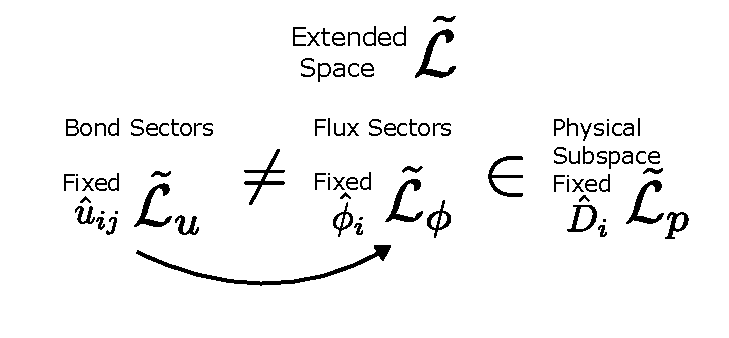
\includegraphics[width=1\textwidth,height=\textheight]{figure_code/amk_chapter/hilbert_spaces}
\caption[{How the different Hilbert Spaces relate to one another}]{The relationship between the different Hilbert spaces used in the solution. \textbf{needs updating}}
\label{fig:hilbert_spaces}
\end{figure}
}

The physical states are defined as those for which \(D_i |\phi\rangle = |\phi\rangle\) for all \(D_i\). Since \(D_i\) has eigenvalues \(\pm1\), the quantity \(\tfrac{(1+D_i)}{2}\) has eigenvalue \(1\) for physical states and \(0\) for extended states so is the local projector onto the physical subspace.

Therefore, the global projector is \[ \mathcal{P} = \prod_{i=1}^{2N} \left( \frac{1 + D_i}{2}\right)\]

for a toroidal trivalent lattice with \(N\) plaquettes \(2N\) vertices and \(3N\) edges. As discussed earlier, the product over \((1 + D_j)\) can also be thought of as the sum of all possible subsets \(\{i\}\) of the \(D_j\) operators, which is the set of all possible gauge symmetry operations.

\[ \mathcal{P} = \frac{1}{2^{2N}} \sum_{\{i\}} \prod_{i\in\{i\}} D_i\]

Since the gauge operators \(D_j\) commute and square to one, we can define the complement operator \(C = \prod_{i=1}^{2N} D_i\) and see that it takes each set of \(\prod_{i \in \{i\}} D_j\) operators and gives us the complement of that set. We will shortly see why \(C\) is the identity in the physical subspace, as noted earlier.

We use the complement operator to rewrite the projector as a sum over half the subsets of \(\{i\}\) - referred to as \(\Lambda\). The complement operator deals with the other half

\[ \mathcal{P} =  \left( \frac{1}{2^{2N-1}} \sum_{\Lambda} \prod_{i\in\{i\}} D_i\right) \left(\frac{1 + \prod_i^{2N} D_i}{2}\right) = \mathcal{S} \cdot \mathcal{P}_0\]

To compute \(\mathcal{P}_0\), the main quantity needed is the product of the local projectors \(D_i\) \[\prod_i^{2N} D_i = \prod_i^{2N} b^x_i b^y_i b^z_i c_i \] for a toroidal trivalent lattice with \(N\) plaquettes \(2N\) vertices and \(3N\) edges.

First, we reorder the operators by bond type. This does not require any information about the underlying lattice.

\[\prod_i^{2N} D_i = \prod_i^{2N} b^x_i \prod_i^{2N} b^y_i \prod_i^{2N} b^z_i \prod_i^{2N} c_i\]

The product over \(c_i\) operators reduces to a determinant of the Q matrix and the fermion parity, see~\autocite{pedrocchiPhysicalSolutionsKitaev2011}. The only difference from the honeycomb case is that we cannot explicitly compute the factors \(p_x,p_y,p_z = \pm\;1\) that arise from reordering the b operators such that pairs of vertices linked by the corresponding bonds are adjacent.

\[\prod_i^{2N} b^\alpha_i = p_\alpha \prod_{(i,j)}b^\alpha_i b^\alpha_j\]

However, they are simply the parity of the permutation from one ordering to the other and can be computed in linear time with a cycle decomposition~\autocite{sedgewickPermutationGenerationMethods1977}.

We find that \[\mathcal{P}_0 = 1 + p_x\;p_y\;p_z\; \hat{\pi} \; \mathrm{det}(Q^u) \; \prod_{\{i,j\}} -iu_{ij}\]

where \(p_x\;p_y\;p_z = \pm 1\) are lattice structure factors and \(\mathrm{det}(Q^u)\) is the determinant of the matrix mentioned earlier that maps \(c_i\) operators to normal mode operators \(b'_i, b''_i\). These depend only on the lattice structure.

\(\hat{\pi} = \prod{i}^{N} (1 - 2\hat{n}_i)\) is the parity of the particular many-body state determined by fermionic occupation numbers \(n_i\). As discussed in~\autocite{pedrocchiPhysicalSolutionsKitaev2011}, \(\hat{\pi}\) is gauge invariant in the sense that \([\hat{\pi}, D_i] = 0\).

This implies that \(det(Q^u) \prod -i u_{ij}\) is also a gauge invariant quantity. In translation invariant models this quantity which can be related to the parity of the number of vortex pairs in the system~\autocite{yaoAlgebraicSpinLiquid2009}.

All these factors take values \(\pm 1\) so \(\mathcal{P}_0\) is 0 or 1 for a particular state. Since \(\mathcal{S}\) corresponds to symmetrising over all the gauge configurations and cannot be 0, once we have determined the single particle eigenstates of a bond sector, the true many-body ground state has the same energy as either the empty state with \(n_i = 0\) or a state with a single fermion in the lowest level.
